% !TEX TS-program = pdflatex
% !TEX encoding = UTF-8 Unicode


\documentclass[11pt]{article} % use larger type; default would be 10pt

\usepackage[utf8]{inputenc} % set input encoding (not needed with XeLaTeX)
\usepackage[portuges]{babel}


%%% PAGE DIMENSIONS
\usepackage{a4}

\usepackage{graphicx} % support the \includegraphics command and options

%%% PACKAGES
\usepackage{booktabs} % for much better looking tables
\usepackage{array} % for better arrays (eg matrices) in maths
\usepackage{paralist} % very flexible & customisable lists (eg. enumerate/itemize, etc.)
\usepackage{verbatim} % adds environment for commenting out blocks of text & for better verbatim
\usepackage{subfig} % make it possible to include more than one captioned figure/table in a single float
% These packages are all incorporated in the memoir class to one degree or another...

%%% HEADERS & FOOTERS
\usepackage{fancyhdr} % This should be set AFTER setting up the page geometry
\pagestyle{fancy} % options: empty , plain , fancy
\renewcommand{\headrulewidth}{0pt} % customise the layout...
\lhead{}\chead{}\rhead{}
\lfoot{}\cfoot{\thepage}\rfoot{}

%%% SECTION TITLE APPEARANCE
\usepackage{sectsty}
\allsectionsfont{\sffamily\mdseries\upshape} % (See the fntguide.pdf for font help)
% (This matches ConTeXt defaults)

%%% ToC (table of contents) APPEARANCE
\usepackage[nottoc,notlof,notlot]{tocbibind} % Put the bibliography in the ToC
\usepackage[titles,subfigure]{tocloft} % Alter the style of the Table of Contents
\renewcommand{\cftsecfont}{\rmfamily\mdseries\upshape}
\renewcommand{\cftsecpagefont}{\rmfamily\mdseries\upshape} % No bold!

%%% END Article customizations

%%% The "real" document content comes below...

\title{Projeto de DSS \\ \large ConfiguraFácil - 1ª Fase}
\date{2018/19}

\begin{document}
\maketitle

\begin{table}[!htbp]
\centering
\begin{tabular}{cc}
 Diogo Sobral (a82523) &  Henrique Pereira (a80261) \\
 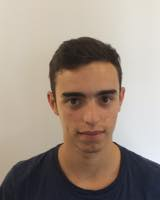
\includegraphics[height=0.8in]{Diogo} &  
\includegraphics[height=0.8in]{Henrique} \\
	& \\
 Pedro Moreira (a82364)  &   Pedro Ferreira (a81135) \\
 
\includegraphics[height=0.8in]{PedroM} & 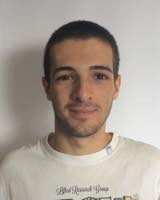
\includegraphics[height=0.8in]{PedroF} \\

\end{tabular}
\end{table}

\newpage
\tableofcontents
\newpage

\section{Introdução}


\section{Diagrama de Domínio}


\section{Diagrama de Use Cases}

\section{Especificação de Use Cases}

\section{Protótipo de Interface}

\section{Diagrama de Máquinas de Estado}


\end{document}
